\documentclass[10pt]{article}
\usepackage[margin=0.62in]{geometry}
\usepackage[T1]{fontenc}
\usepackage[utf8]{inputenc}
\usepackage[american]{babel}
\usepackage{lmodern}
\usepackage{microtype}
\usepackage{parskip}
\usepackage{setspace}
\usepackage{amsmath,amssymb}
\usepackage{booktabs,tabularx,array}
\usepackage{graphicx}
\usepackage{float}
\usepackage{xcolor}
\usepackage{tikz}
\usetikzlibrary{arrows.meta,positioning,calc,fit}
\usepackage{multicol}
\usepackage[round,authoryear]{natbib}
\usepackage[hidelinks]{hyperref}

\definecolor{accent}{HTML}{0F6D67}
\definecolor{ink}{HTML}{17202A}
\definecolor{soft}{HTML}{EEF4F3}
\definecolor{warm}{HTML}{F6F2EA}
\hypersetup{colorlinks=true,citecolor=accent,urlcolor=accent,linkcolor=accent}
\setstretch{0.965}
\setlength{\parskip}{3.5pt}
\setlength{\parindent}{0pt}
\setlength{\columnsep}{12pt}
\pagestyle{empty}

\newcommand{\sectionbar}[1]{%
  \section*{\color{ink}#1}\vspace{-4pt}}
\newcommand{\tightcite}[1]{\citep{#1}}
\newcommand{\facetimg}[1]{%
  \includegraphics[width=1.40in,trim=0 400 0 0,clip]{#1}}

\begin{document}

\begin{center}
{\LARGE\bfseries Politics of Appearance}\par
\vspace{2pt}
{\large\bfseries A Matched-Identity Candidate Experiment in Finland and Chile}\par
\vspace{5pt}
{\normalsize Outi Sarpila \quad $\cdot$ \quad H\'ector Bahamonde \quad $\cdot$ \quad Nayssa Alejandra Mar\'in D\'iaz}\par
\end{center}

\vspace{-2pt}
\begin{center}
\begin{minipage}{0.94\linewidth}
\colorbox{soft}{\parbox{0.965\linewidth}{%
\textbf{Abstract.} Citizens routinely encounter political candidates first as images. This study identifies whether modifiable political self-presentation---clothing, grooming, hair arrangement, and accessories---causally shapes candidate choice and trait evaluation, and whether those effects depend on congruence with stated policy. Four fictional Finnish identities are each rendered in progressive-coded, neutral, and conservative-coded forms while identity, expression, pose, lighting, age, and background remain fixed. In two paired municipal-election tasks, appearance, economic policy, and sociocultural policy are independently randomized. The design therefore separates an appearance effect from stable facial identity and from the political information attached to the image.}}
\end{minipage}
\end{center}

\vspace{-1pt}
\begin{center}
\fcolorbox{accent}{warm}{\parbox{0.89\linewidth}{\centering
\textbf{\color{accent}Prototype:}\quad
\href{https://political-appearance-finland.onrender.com}{\texttt{political-appearance-finland.onrender.com}}
}}
\end{center}
\vspace{-3pt}

\sectionbar{Motivation and contribution}
Facial and bodily appearance can serve as a ``heuristic'' \tightcite{tversky1974}, a rapid (political) cue, particularly when information is limited. Yet appearance is not a neutral measurement device: attractiveness and competence create halo effects in perceived ideology \tightcite{herrmann2016}; stereotypically conservative-looking faces can affect candidate support \tightcite{olivola2018}; and a dominant-looking face can help with conservative audiences while backfiring among liberals \tightcite{laustsen2016}. Appearance also communicates social position. In Finnish municipal elections, upper-class-looking candidates received more votes, while working-class-looking women faced a distinctive penalty \tightcite{bahamonde2024}. These findings imply that the same look need not be universally advantageous. Its meaning should depend on the political message, the audience, and the status boundaries active in a society.

This experiment advances this literature by manipulating \emph{self-presentation within identity}. It asks whether politically coded appearance changes (i) vote choice; (ii) trustworthiness, competence, credibility, authenticity, and political suitability; (iii) perceived ideology; and (iv) perceived appearance--policy fit. Independent randomization turns a multidimensional image-and-policy profile into a ``visual'' conjoint experimental design \tightcite{hainmueller2014,vecchiato2025}. Unlike a text-only profile-like conjoint design, the treatment in the current design preserves the visual mode in which candidates are commonly encountered.

\sectionbar{Design and hypotheses}
Four identity-locked portrait triptychs yield $4\times3=12$ image files. Respondents see two nonrepeating pairs: identities 1--2 in Task 1 and identities 3--4 in Task 2. Appearance $A\in\{-1,0,+1\}$ denotes progressive-coded, neutral, or conservative-coded presentation. Economic policy $E\in\{-1,+1\}$ and sociocultural policy $S\in\{-1,+1\}$ are independently randomized, as are screen side and the profile rated after each forced-choice vote (see \autoref{fig:design}).

\textbf{H1:} Appearance shifts perceived ideology after policy information is shown. \textbf{H2:} appearance--platform congruence increases vote probability, credibility, authenticity, political suitability, and perceived fit. \textbf{H3:} effects vary with respondent ideology, class, knowledge, candidate gender, and country.


\sectionbar{Causal logic}
For respondent $i$, candidate $j$, and task $t$, let $Y_{ijt}(a,e,s)$ denote a potential outcome under appearance $a$, economic policy $e$, and sociocultural policy $s$, with identity $j$ held fixed. The appearance AMCE relative to neutral is
\[
\tau_a=\mathbb{E}_{E,S,J,T}\!\left[Y_{ijt}(a,E,S)-Y_{ijt}(0,E,S)\right],\quad a\in\{-1,+1\}.
\]
For coherent platforms, let $P=-1$ denote economic-left/cultural-liberal and $P=+1$ economic-right/cultural-conservative. The appearance--platform interaction is
\[
\tau_{G}=\{\mu(+1,+1)-\mu(-1,+1)\}
-\{\mu(+1,-1)-\mu(-1,-1)\},
\]
where $\mu(a,p)=\mathbb{E}[Y\mid A=a,P=p]$. Random assignment identifies both quantities; standard errors cluster by respondent and identity in the comparative study.

\begin{center}
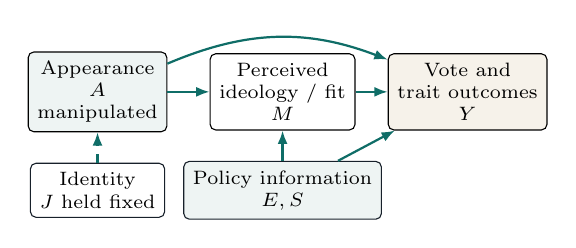
\begin{tikzpicture}[
 n/.style={draw,rounded corners=2pt,align=center,minimum width=1.55cm,minimum height=.62cm,font=\scriptsize},
 a/.style={-{Latex[length=1.7mm]},draw=accent,thick},
 c/.style={draw=ink,rounded corners=2pt,align=center,minimum width=1.55cm,minimum height=.62cm,font=\scriptsize}
]
\node[n,fill=soft] (A) at (0,0) {Appearance\\$A$\\\scriptsize manipulated};
\node[n] (M) at (2.35,0) {Perceived\\ideology / fit\\$M$};
\node[n,fill=warm] (Y) at (4.7,0) {Vote and\\trait outcomes\\$Y$};
\node[c,fill=soft] (P) at (2.35,-1.25) {Policy information\\$E,S$};
\node[c] (J) at (0,-1.25) {Identity\\$J$ held fixed};
\draw[a] (A)--(M); \draw[a] (M)--(Y); \draw[a] (A) to[bend left=22] (Y);
\draw[a] (P)--(M); \draw[a] (P)--(Y); \draw[a,dashed] (J)--(A);
\end{tikzpicture}

{\scriptsize Causal pathway and design control.}
\end{center}



\sectionbar{Experimental contribution}
The experiment uses identity-matched images, independently randomizes appearance and two policy dimensions, prevents within-person identity repetition, randomizes the rated profile, and exports every assignment with choice time and outcomes. The three appearance conditions will be independently validated to establish their perceived political meanings in Finland and Chile.

Before fielding, a Finnish pretest must assess perceived ideology, class/status, attractiveness, apparent age, gender expression, realism, AI artifacts, and resemblance to real people. Selection rules and exclusions should be preregistered: synthetic faces can appear unusually trustworthy \tightcite{nightingale2022}, while generators can reproduce stereotypes and homogenize groups \tightcite{aldahoul2025}.

\sectionbar{Why it matters}
The design distinguishes appearance from facial identity and tests whether visual presentation corroborates or contradicts political substance. Scaling the identity pool in Finland and Chile reveals whether political appearance is a shared heuristic or a context-dependent route through which classed and gendered boundaries enter representation.


\begin{figure}[H]
\centering

\includegraphics[width=0.48\linewidth]{/Users/hectorbahamonde/research/Politics_of_appearance/output/pdf/design.jpeg}
\caption{Candidate-choice task interface (example of one randomization).}
\label{fig:design}
\end{figure}

\sectionbar{Candidate appearance stimuli}
\begin{center}
\setlength{\tabcolsep}{4pt}
\renewcommand{\arraystretch}{0.96}
\begin{tabular}{@{}>{\bfseries\small}r c c c@{}}
 & {\scriptsize\bfseries Progressive-coded} & {\scriptsize\bfseries Neutral} & {\scriptsize\bfseries Conservative-coded} \\
Candidate 1 & \facetimg{/Users/hectorbahamonde/research/Politics_of_appearance/_static/appearance_experiment/images/candidates/candidate_01_v1.png} & \facetimg{/Users/hectorbahamonde/research/Politics_of_appearance/_static/appearance_experiment/images/candidates/candidate_01_v2.png} & \facetimg{/Users/hectorbahamonde/research/Politics_of_appearance/_static/appearance_experiment/images/candidates/candidate_01_v3.png} \\
Candidate 2 & \facetimg{/Users/hectorbahamonde/research/Politics_of_appearance/_static/appearance_experiment/images/candidates/candidate_02_v1.png} & \facetimg{/Users/hectorbahamonde/research/Politics_of_appearance/_static/appearance_experiment/images/candidates/candidate_02_v2.png} & \facetimg{/Users/hectorbahamonde/research/Politics_of_appearance/_static/appearance_experiment/images/candidates/candidate_02_v3.png} \\
Candidate 3 & \facetimg{/Users/hectorbahamonde/research/Politics_of_appearance/_static/appearance_experiment/images/candidates/candidate_03_v1.png} & \facetimg{/Users/hectorbahamonde/research/Politics_of_appearance/_static/appearance_experiment/images/candidates/candidate_03_v2.png} & \facetimg{/Users/hectorbahamonde/research/Politics_of_appearance/_static/appearance_experiment/images/candidates/candidate_03_v3.png} \\
Candidate 4 & \facetimg{/Users/hectorbahamonde/research/Politics_of_appearance/_static/appearance_experiment/images/candidates/candidate_04_v1.png} & \facetimg{/Users/hectorbahamonde/research/Politics_of_appearance/_static/appearance_experiment/images/candidates/candidate_04_v2.png} & \facetimg{/Users/hectorbahamonde/research/Politics_of_appearance/_static/appearance_experiment/images/candidates/candidate_04_v3.png}
\end{tabular}
\vspace{3pt}

\begin{minipage}{0.86\linewidth}
\small\color{ink}\centering
Four identity-matched candidates across all three appearance conditions. The crop emphasizes the face, hair, accessories, and upper-body presentation used as visual cues. Condition labels are analytic and are never shown to respondents.
\end{minipage}
\end{center}


\begin{multicols}{2}
\footnotesize
\begin{thebibliography}{99}
\setlength{\itemsep}{0pt}\setlength{\parskip}{0pt}
\bibitem[AlDahoul et~al.(2025)]{aldahoul2025} AlDahoul, N., Rahwan, T., \& Zaki, Y. (2025). AI-generated faces influence gender stereotypes and racial homogenization. \emph{Scientific Reports}, 15, 14449. \href{https://doi.org/10.1038/s41598-025-99623-3}{doi:10.1038/s41598-025-99623-3}.
\bibitem[Bahamonde and Sarpila(2024)]{bahamonde2024} Bahamonde, H., \& Sarpila, O. (2024). Physical appearance and elections: An inequality perspective. \emph{Political Psychology}, 45, 623--642. \href{https://doi.org/10.1111/pops.12940}{doi:10.1111/pops.12940}.
\bibitem[Hainmueller et~al.(2014)]{hainmueller2014} Hainmueller, J., Hopkins, D. J., \& Yamamoto, T. (2014). Causal inference in conjoint analysis. \emph{Political Analysis}, 22, 1--30. \href{https://doi.org/10.1093/pan/mpt024}{doi:10.1093/pan/mpt024}.
\bibitem[Herrmann and Shikano(2016)]{herrmann2016} Herrmann, M., \& Shikano, S. (2016). Attractiveness and facial competence bias face-based inferences of candidate ideology. \emph{Political Psychology}, 37, 401--417. \href{https://doi.org/10.1111/pops.12256}{doi:10.1111/pops.12256}.
\bibitem[Laustsen and Petersen(2016)]{laustsen2016} Laustsen, L., \& Petersen, M. B. (2016). Winning faces vary by ideology. \emph{Political Communication}, 33, 188--211. \href{https://doi.org/10.1080/10584609.2015.1050565}{doi:10.1080/10584609.2015.1050565}.
\bibitem[Nightingale and Farid(2022)]{nightingale2022} Nightingale, S. J., \& Farid, H. (2022). AI-synthesized faces are indistinguishable from real faces and more trustworthy. \emph{PNAS}, 119, e2120481119. \href{https://doi.org/10.1073/pnas.2120481119}{doi:10.1073/pnas.2120481119}.
\bibitem[Olivola et~al.(2018)]{olivola2018} Olivola, C. Y., Tingley, D., \& Todorov, A. (2018). Republican voters prefer candidates who have conservative-looking faces. \emph{Political Psychology}, 39, 1157--1171. \href{https://doi.org/10.1111/pops.12489}{doi:10.1111/pops.12489}.
\bibitem[Vecchiato and Munger(2025)]{vecchiato2025} Vecchiato, A., \& Munger, K. (2025). Introducing the visual conjoint. \emph{Journal of Experimental Political Science}, 12, 57--71. \href{https://doi.org/10.1017/XPS.2024.15}{doi:10.1017/XPS.2024.15}.
\bibitem[Tversky and Kahneman(1974)]{tversky1974}
Tversky, A., \& Kahneman, D. (1974).
Judgment under uncertainty: Heuristics and biases.
\emph{Science}, 185(4157), 1124--1131.
\href{https://doi.org/10.1126/science.185.4157.1124}{doi:10.1126/science.185.4157.1124}.
\end{thebibliography}
\end{multicols}

\end{document}
